\documentclass[10pt,twocolumn,letterpaper]{article}

\usepackage{cvpr}
\usepackage{times}
\usepackage{epsfig}
\usepackage{graphicx}
\usepackage{amsmath}
\usepackage{amssymb}

% Include other packages here, before hyperref.

% If you comment hyperref and then uncomment it, you should delete
% egpaper.aux before re-running latex.  (Or just hit 'q' on the first latex
% run, let it finish, and you should be clear).
\usepackage[breaklinks=true,bookmarks=false]{hyperref}

\cvprfinalcopy % *** Uncomment this line for the final submission

\def\cvprPaperID{****} % *** Enter the CVPR Paper ID here
\def\httilde{\mbox{\tt\raisebox{-.5ex}{\symbol{153}}}}

% Pages are numbered in submission mode, and unnumbered in camera-ready
%\ifcvprfinal\pagestyle{empty}\fi
\setcounter{page}{1}
\begin{document}

%%%%%%%%% TITLE
\title{Pedestrian Detection Using Correlated Lidar and Image Data}

\author{Samuel Rohrer\\
University of Michigan\\
{\tt\small rohrer@umich.edu}
% For a paper whose authors are all at the same institution,
% omit the following lines up until the closing ``}''.
% Additional authors and addresses can be added with ``\and'',
% just like the second author.
% To save space, use either the email address or home page, not both
\and
Ian Lin\\
University of Michigan\\
{\tt\small tiannis@umich.edu}
}

\maketitle
%\thispagestyle{empty}

%%%%%%%%% ABSTRACT
\begin{abstract}
  Recent progress in software and hardware systems will lead to an increase in
  daily interactions with robots and intelligent systems. As a result of this 
  safety must be at the forefront of the design of autonomous systems, 
  particularly autonomous cars. With this in mind we aim to create a pedestrian
  detection system based off of sensors commonly found on autonomous vehicles.
  We will use correlated Lidar and image data along with algorithms found in 
  recent papers to perform pedestrian detection.

\end{abstract}

%%%%%%%%% BODY TEXT
\section{Introduction}

  As progress in software and hardware continues, it is expected that 
  autonomous robotics and intelligent systems will begin to play an integral 
  role in everyday life. Jobs that are physically demanding or unsafe can be 
  replaced by robots and autonomous cars can greatly improve road safety and
  efficiency. In order for these intelligent systems to succeed, safety must 
  be at the forefront of their design. Detection of obstacles is a very
  significant aspect of this concern, especially for autonomous cars which
  must detect not only other cars, but also road signs, traffic signals, and
  pedestrians. In particular, pedestrian detection is an ongoing research
  area within computer vision.

  The goal of this project is to detect pedestrians in a pre-existing dataset: 
  the LIPD dataset provides correlated LIDAR data and image data. We aim to do
  this by identifying obstacles on the road, based on LIDAR data, and
  associating these obstacles to the image data through feature extraction.
  After feature extraction, we plan to use a trained classifier to determine
  if the obstacle is indeed a pedestrian in the road. We could extend this by 
  training a more sophisticated classifier that has the ability to discern the 
  difference between cars, pedestrians, and road signs.

%------------------------------------------------------------------------
\section{Previous Work}

  There has been a good deal of work in the area of pedestrian detection for 
  mobile robotics. In most systems, the sensor subsystems operate independently
  of each other. In \cite{journal} the authors use Lidar to generate regions
  of interest, then use image analysis to determine the presence of a 
  pedestrian. Some other sensors available on modern autonomous robotics 
  platforms include: radar, ultrasound, camera sensors and Lidar (light
  detection and ranging). However, each of these sensors comes with their own
  inherent problems. Cameras can fail in low light situations, and Lidar can
  fail when objects are side by side at the same distance. Both can fail in poor
  weather, as Lidar can fail if rain or snow causes the light to be reflected
  too early and camera images can fail if the lens is obstructed by poor weather.

  In order to complete this project, we started with a data set \cite{dataset}.
  Some benefits of this dataset include: correlated Lidar and image data, and 
  a classification dataset. The correlated datasets were composed of a forward
  facing camera (limited field of view relative to Lidar) and four Lidar scans
  all facing outwards at different angles. The classification dataset had both
  training and testing sets for the Lidar.


%------------------------------------------------------------------------
\section{Technical Work}

  We plan to use both the Lidar data and image data together to identify 
  pedestrians on the road. With Lidar data, we can identify obstacles on the 
  road and then analyze the corresponding images that potentially contain 
  pedestrians. There has already been work done in the areas of correlating 
  Lidar and single image data for the purpose of detecting pedestrians. Most 
  of it follows the same approach that we are outlining and has had succes. 
  For Lidar object detection, we decided to follow the pipeline outlined 
  in \cite{journal}, and add stages for error correction and correlation with 
  image data. The pipeline is as follows: segmentation, feature
  extraction, classification, error correction, and correlation with image data.
  
  \subsection{Lidar Segmentation}
  The pipeline begins with segmentation of the Lidar data 
  to find the points where the directionality of the segment changes. 
  According to \cite{conf} if it 
  is a new segment then (1) holds true where $r_i$ is the 
  distance to current point, $r_{i+1}$ is the distance to next point, 
  $cos(\Delta \alpha)$ is the 3D angle between the two points, and $C_0$ is a 
  constant to adjust for noise:
   \begin{equation} \sqrt{r_{i}^{2} + r_{i+1}^{2} - 2 r_{i} r_{i+1}
   cos(\Delta \alpha)} > thd \end{equation}
   \begin{equation} thd = C_0 + \sqrt{2(1-cos(\Delta \alpha} * min(r_i,
   r_{i+1}) \end{equation}

  For the purpose of this project any segment less than three points long was 
  discarded before moving to feature extraction. This was performed for each 
  Lidar scan in isolation of the other scans. 

  \subsection{Feature Extraction}
  After separating the Lidar scan data into different segments we then 
  performed feature extraction on the segments. We used 10 different features 
  for each segment, based on \cite{journal}.

  \renewcommand{\arraystretch}{1.5}
  \begin{center}
    \begin{tabular}{ | p{1cm} | l | p{2.9cm} |}
      \hline
      Feature num & Formula & Description \\ \hline
      1 & $ np $ & number range points \\ \hline
      2 & $np*r_{min}$ & number of range points * minimum range distance \\ \hline
      3 & $\sqrt{ \Delta X^2 + \Delta Y^2} $ & RMS of segment width and height
      \\ \hline
      4 & $ \frac{1}{np}\sum_{n=1}^{np} || x_n - x_m|| $ & Mean average deviation
      from median ($x_m$) \\ \hline
      5 & $ \frac{1}{np}\sum_{n=1}^{np} (x_n - x_{lsq})^2 $ & Linearity - 
      distance to the least squares line ($ x_{lsq}$) \\ \hline
      6 & $ \frac{1}{np}\sum_{n=1}^{np} (x_n - \mu_x)^2 $ & Second central 
      moment (about mean $\mu_x$) \\ \hline
      7 & $ \frac{1}{np}\sum_{n=1}^{np} (x_n - \mu_x)^3 $ & Third central 
      moment (about mean $\mu_x$) \\ \hline
      8 & $ \frac{1}{np}\sum_{n=1}^{np} (x_n - \mu_x)^4 $ & Fourth central 
      moment (about mean $\mu_x$) \\ \hline
      9 & $ \sum_{n=1}^{np} ||x_n - x_{n-1}|| $ & Segment length (norm distance
      between points) \\ \hline
      10 & $ \sigma(ft9) $ & Standard deviation of
      segment length (norm distance between points) \\ \hline
    \end{tabular}
  \end{center}

  These features were all able to be computed quickly and robustly for all 
  segments greater than three points long.

  \subsection{Classification}
  For classification we used training data from \cite{dataset} to determine 
  which features corresponded to a pedestrian. To implement this classifier
  we used Python's SkLearn DecisionTreeClassifier \cite{sklearn}. 
  It was trained on the labeled pedestrian segments from the training set.
  On very clean, well segmented data (also available from \cite{journal})
  our classifier has an accuracy of 88%.

  \subsection{Error Correction}
  Our initial results were somewhat prone to error, as seen in Figure 1.
  \begin{figure}
    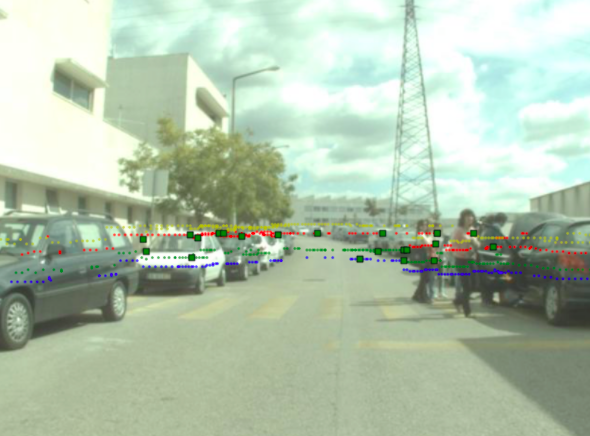
\includegraphics[height=2.8in, width=3.5in]{images/initial_result.png}
    \caption{ Initial segmentation results. Green squares are identified 
    segments. Red, blue, yellow and green dots are Lidar points.}
  \end{figure}

  To account for this error, we decided to only classify a pedestrian from the 
  Lidar data if we found at least three identifications across Lidar scans 
  (out of four Lidar scans) within a 50 pixel margin. Results of this will be 
  discussed in the Experimental Results section.

  \subsection{Correlation with Image Data}
  In order to create a classifier even better than the one proposed in 
  \cite{journal} we decided to add another check before positively identifying 
  a pedestrian. To do this we modified the peopledetect.py sample file from
  OpenCV \cite{opencv} to return the bounding boxes of all pedestrians instead
  of just drawing them. Then if the Lidar classifier with error correction and 
  the OpenCV classifier both classified a pedestrian we said that a pedestrian
  was in fact present in the image.


%------------------------------------------------------------------------
\section{Experimental Results}


%------------------------------------------------------------------------
\section{Conclusion}


%------------------------------------------------------------------------

{\small
\bibliographystyle{ieee}
\bibliography{egbib}
}

\end{document}
